% ====================================================================
\section{Theory}\label{sec:theory}
% ====================================================================

\subsection{Resonance condition}\label{sec:resonance}

The spin $\vec S$ of an electron carries the magnetic moment $\vec\mu=-g\muB\vec S/\hbar$, with the Bohr magneton
$\muB$ and the $g$-factor ($g_\mathrm e=\num{2.0023}$ for the free electron). Because of the negative charge, moment
and spin point in opposite directions. In a field $B$ the state with spin projection
$m_S=\pm\frac12$ has the energy $E=g\muB Bm_S$, and the two levels are $\Delta E=g\muB B$ apart (Zeeman effect).
An alternating magnetic field $B_1$ of frequency $\nu$, perpendicular to $B$, can flip the spin if the photon energy
matches the splitting:
\begin{equation}\label{eq:resonance}
  h\nu=g\muB\Br
  \qquad\Longleftrightarrow\qquad
  g=\frac{h}{\muB}\,\frac{\nu}{\Br},\qquad \frac{h}{\muB}=\qty{71.4477}{mT/GHz}.
\end{equation}
At $\nu=\qty{9.36}{GHz}$ and $g\approx2$ the resonance lies at $\Br\approx\qty{334}{mT}$. Classically,
the moment precesses about the field at the Larmor frequency $\omega_0=\gamma B$, with $\gamma=g\muB/\hbar$. At resonance
the alternating field rotates in step with this precession and can keep tilting the spin. Both pictures
give the same condition.

The $g$-factor deviates from $g_\mathrm e$ when spin-orbit coupling mixes some orbital moment into the spin. For the
organic radical DPPH the deviation is tiny ($g=\num{2.0036}$). The same holds for \ce{Mn^2+}, whose five d electrons
together have no orbital moment ($L=0$). Dilute samples give $g=\numrange{2.000}{2.002}$~\cite{abragam1970}.

The microwave drives transitions up and down equally strongly. A sample absorbs net energy only because the lower
level is slightly more populated than the upper one. At room temperature the Boltzmann excess is
$(N_--N_+)/N=\tanh(h\nu/2\kB T)\approx\num{7.6e-4}$, less than one part per thousand. The signal is
small, and the whole setup (\cref{sec:detection,sec:modulation}) is built to make it visible anyway.

\subsection{Line shape and \texorpdfstring{$T_2$}{T2}}\label{sec:lineshape}

The resonance has a finite width. After an excitation the spins first precess together and form a
rotating transverse magnetization. But each spin feels a slightly different local field from its neighbors, so the
precessions drift out of phase. The transverse magnetization decays in the time $T_2$ (spin-spin relaxation). The
level populations also relax to thermal equilibrium in the time $T_1$ by giving energy to the crystal
lattice (spin-lattice relaxation). The Bloch equations describe both processes:
\begin{equation}\label{eq:bloch}
  \dot{\vec M}=-\gamma\,\vec M\times\vec B-\frac{M_x\hat x+M_y\hat y}{T_2}-\frac{M_z-M_0}{T_1}\,\hat z .
\end{equation}
In the steady state the magnetization responds to the microwave field with a complex susceptibility
$\chi=\chiI-\ii\chiII$. $\chiII$ is \ang{90} out of phase with the field and takes energy from it
(\emph{absorption}). $\chiI$ oscillates in phase and stores energy only temporarily (\emph{dispersion}). The
experiment sweeps the field at fixed frequency. With $x=(B-\Br)/\Bhalf$ the solution is
\begin{equation}\label{eq:chi}
  \chiII\propto\frac{1}{1+x^2+s},\qquad \chiI\propto\frac{x}{1+x^2+s},\qquad
  \Bhalf=\frac{1}{\gamma T_2},\qquad s=\gamma^2B_1^2T_1T_2 .
\end{equation}
The absorption is a Lorentzian line whose half width at half maximum (HWHM) $\Bhalf$ is inversely proportional to $T_2$.
As for any damped oscillation, the shorter the spins stay in phase, the less sharp their frequency.
The parameter $s$ describes saturation. If $B_1$ is so large that the microwave flips the spins faster than
relaxation in the time $T_1$ restores equilibrium ($s\gtrsim1$), the populations equalize. The absorption then no
longer grows with the power, and the line broadens by the factor $\sqrt{1+s}$.

\subsection{Broad lines in concentrated samples}\label{sec:width}

In DPPH and \ce{MnCl2} the spins are densely packed, and each spin feels the dipolar fields of its neighbors. In
\ce{MnCl2} the six nearest neighbors alone produce about \qty{0.2}{T}~\cite{vanvleck1948}. If
these fields were static, each spin would have its own resonance frequency, giving a roughly Gaussian line
with an HWHM of about \qty{0.25}{T}.

Neighboring spins are also coupled by exchange, a result of Coulomb repulsion and the
Pauli principle. Exchange lets the spin orientations hop between
neighbors at a rate $\omega_\mathrm e$ without shifting the overall resonance. The local field
at a spin then fluctuates rapidly, and on average the spin sees only the external field. If this
hopping is fast compared with the frequency spread from the dipolar fields, the line becomes narrow and
Lorentzian~\cite{anderson1953}:
\begin{equation}\label{eq:aw}
  \Bhalf\approx\frac{M_2}{B_\text{ex}},\qquad B_\text{ex}=\frac{\omega_\mathrm e}{\gamma},
\end{equation}
where $\sqrt{M_2}$ is the width of the static dipolar field distribution. This is exchange narrowing.
In NMR of liquids, molecular motion averages out the dipolar fields in the same way. Exchange
also wipes out the hyperfine structure. Because of the nuclear spin $I=\frac52$ of \ce{^{55}Mn}, dilute \ce{Mn^2+}
shows six lines about \qty{9.5}{mT} apart. In pure \ce{MnCl2} the excitation moves from ion to ion too quickly, and
only one line remains. The DPPH line is also exchange-narrowed and very narrow, a few tenths of a millitesla.

\subsection{Detection: cavity, bridge and waveguide}\label{sec:detection}

\begin{figure}[t]
  \centering
  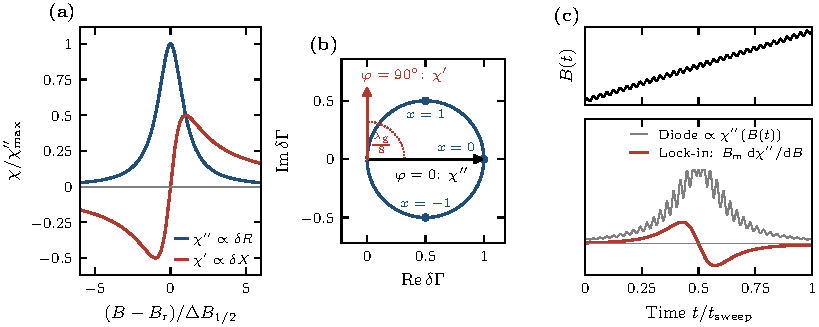
\includegraphics[width=\textwidth]{figures/theory.pdf}
  \caption{Calculated curves (no measurements) for the preparatory exercises. (a)~Absorption $\chiII$ and dispersion
  $\chiI$ of a Lorentzian line versus field. The cavity changes its resistance by $\delta R\propto\chiII$ and its
  reactance by $\delta X\propto\chiI$ (\cref{eq:rx}). (b)~As the field passes through resonance, the change
  $\delta\Gamma\propto\chiII+\ii\chiI$ of the reflected wave traces a circle ($x=(B-\Br)/\Bhalf$). The diode sees only
  its projection onto the reference phase $\varphi$. With $\varphi=0$ it sees absorption, with $\varphi=\ang{90}$
  dispersion. The two settings are a plunger travel of $\lamg/8$ apart. (c)~Field with modulation (top), diode signal
  and lock-in output (bottom), here with $\Bm=\Bhalf/4$ and, for clarity, only 34 modulation periods per sweep.}
  \label{fig:theory}
\end{figure}

\paragraph{Cavity.}
The sample sits in the rectangular cavity (mode TE$_{102}$) where the magnetic microwave field $B_1$ is maximal.
The cavity stores the microwave energy over many oscillations, which enhances the field at the sample. Its
quality factor $\QL\approx930$ corresponds to a resonance width of only $\nu/\QL\approx\qty{10}{MHz}$. Near resonance
the cavity behaves like a series resonant circuit. The sample fills a fraction $\eta$ (filling factor) of the magnetic
field volume and changes the circuit inductance to $L=L_0(1+\eta\chi)$. With
$\chi=\chiI-\ii\chiII$ and the time dependence $e^{\ii\omega t}$ the impedance becomes
\begin{equation}\label{eq:rx}
  Z=R+\ii\omega L_0(1+\eta\chi)+\frac{1}{\ii\omega C}
  \quad\Longrightarrow\quad
  \delta R=\omega L_0\eta\,\chiII,\qquad \delta X=\omega L_0\eta\,\chiI .
\end{equation}

\begin{exercise}{1}
$\chiII$ is a positive Lorentzian with its maximum at resonance (\cref{fig:theory}a). $\chiI$ is positive on one
side of the resonance and negative on the other. It has its extrema at $x=\pm1$, i.e., $\Bhalf$ away from the center,
and further out it falls off only slowly ($\propto1/x$). Since the prefactor $\omega L_0\eta$ is constant during the
field sweep, $\delta R$ follows the absorption exactly and $\delta X$ the dispersion. The sample takes energy from the
cavity, making it lossier, and slightly detunes it. Sweeping the frequency instead of the field gives
exactly the same curves, with $x=(\omega-\omega_0)T_2$.
\end{exercise}

\paragraph{Bridge.}
The signal is the wave reflected by the cavity. If the cavity is coupled so that nothing is reflected at resonance
(critical coupling), the sample produces a small reflected wave
\begin{equation}\label{eq:dgamma}
  \delta\Gamma=\eta\QL\,\bigl(\chiII+\ii\chiI\bigr):
\end{equation}
absorption changes it in phase and dispersion \ang{90} out of phase (\cref{fig:theory}b). On its own this wave
would hardly be measurable, because the diode measures power, $|\delta\Gamma|^2$, the square of a tiny quantity.
A magic T, a waveguide junction with four arms, therefore mixes in a reference wave. The
wave from the source splits between the cavity arm and a reference arm with the attenuator X382A and a movable
short circuit (the \enquote{plunger}). The waves returning from both meet in the fourth arm, where the diode
sits. With $E_c$ the amplitude of the wave at the cavity and $E_be^{\ii\varphi}$ the reference wave at the diode, the
diode measures
\begin{equation}\label{eq:diode}
  V_D\propto\bigl|E_be^{\ii\varphi}+E_c\,\delta\Gamma\bigr|^2
  \approx E_b^2+2E_bE_c\,\eta\QL\bigl(\chiII\cos\varphi+\chiI\sin\varphi\bigr).
\end{equation}
The reference makes the signal linear in $\chi$ and amplifies it by the factor $E_b$. Its phase $\varphi$ selects
absorption, dispersion or a mixture of the two.

\paragraph{Waveguide and plunger.}
The microwave travels in a rectangular waveguide of width $a$. The fundamental mode propagates only if half a
wavelength fits across the width, that is, above the cutoff frequency $\nu_\mathrm c=c/2a$. Above cutoff the wave zigzags
between the walls, and its wavelength along the guide is longer than in free space ($\lambda_0=c/\nu$):
\begin{equation}\label{eq:lamg_theory}
  \lamg=\frac{\lambda_0}{\sqrt{1-(\nu_\mathrm c/\nu)^2}} .
\end{equation}
Moving the plunger by $\Delta z$ lengthens the path of the reference wave by $2\Delta z$, so its phase turns by
$|\Delta\varphi|=4\pi\Delta z/\lamg$.

\begin{exercise}{2}
For $\varphi=0$ the bridge measures $\chiII$ (absorption), for $\varphi=\pm\ang{90}$ it measures $\chiI$ (dispersion).
Switching between them takes a phase change of \ang{90}, so the plunger has to move by $\Delta z=\lamg/8$. For the WR-90
waveguide ($a=\qty{22.86}{mm}$, $\nu_\mathrm c=\qty{6.557}{GHz}$) at $\nu=\qty{9.359}{GHz}$ this gives
$\lamg=\qty{44.89}{mm}$ and $\Delta z=\qty{5.61}{mm}$.
\end{exercise}

\subsection{Field modulation and lock-in}\label{sec:modulation}

The spins change the diode voltage only slightly compared with its bias $E_b^2$, which drifts slowly and
is noisy. So a small modulation $\Bm\cos\omega_\mathrm m t$ with
$\omega_\mathrm m/2\pi=\qty{133}{Hz}$ is added to the field. The diode signal follows the modulation only near
resonance, and the lock-in picks out exactly this part. It multiplies the signal by a reference of the same
frequency and averages over many periods (time constant $\tau$). The output is
$V_\text{out}=\frac12V_sV_r\cos(\psi_r-\psi_s)$, with amplitude $V_s$ and phase $\psi_s$ of the signal and $V_r$, $\psi_r$
of the reference. Everything at other frequencies, including drift and noise, averages out.

\begin{exercise}{3}
$B(t)$ is a slow ramp with a small ripple (\cref{fig:theory}c, top). The diode signal follows
$\chiII(B(t))$, the slowly swept absorption profile with a ripple on top. The ripple amplitude is
proportional to the slope $|\dd\chiII/\dd B|$. On the rising edge the ripple is in phase with the modulation, on the
falling edge in antiphase, and at the line center it vanishes. The lock-in measures its amplitude and sign.
For $\Bm$ small compared with the line width this is
\begin{equation}\label{eq:harmonic}
  V_1(B)\approx\Bm\,\frac{\dd V_D}{\dd B}\propto\Bm\,\frac{\dd\chiII}{\dd B},
\end{equation}
the derivative of the absorption line (\cref{fig:theory}c, bottom). This is why the recorded line shows one positive
and one negative excursion with a zero crossing in the middle instead of a maximum.
\end{exercise}

The extrema of the derivative Lorentzian lie at $\Br\pm\Bhalf/\sqrt3$. Their separation, the peak-to-peak width,
gives $T_2$ directly:
\begin{equation}\label{eq:t2}
  \Bpp=\frac{2}{\sqrt3}\,\Bhalf
  \qquad\Longrightarrow\qquad
  T_2=\frac{2}{\sqrt3\,\gamma\,\Bpp}.
\end{equation}
A larger $\Bm$ gives a larger signal, but only while $\Bm$ is small compared with the line. Once $\Bm$ is comparable to
$\Bpp$, the lock-in averages the derivative over the interval $\pm\Bm$. The measured line gets broader, and the signal
grows more slowly than $\Bm$ (overmodulation). For a Lorentzian, the line is \qty{1}{\percent} too broad at
$\Bm=\Bpp/10$ and already \qty{11}{\percent} too broad at $\Bm=\Bpp/3$. The lab manual therefore recommends $\Bm$
between one fifth and one third of the line width. The sweep must also be slow enough for the low-pass filter of the lock-in
to follow. By a rule of thumb, crossing the line should take at least $10\tau$~\cite{shiroka}.
